\section{Auswertung}
\label{sec:Auswertung}


\subsection{Kennlinien und Sättigungsstrom}
\label{subsec:kennlinien}

\begin{figure}[H]
  \centering
  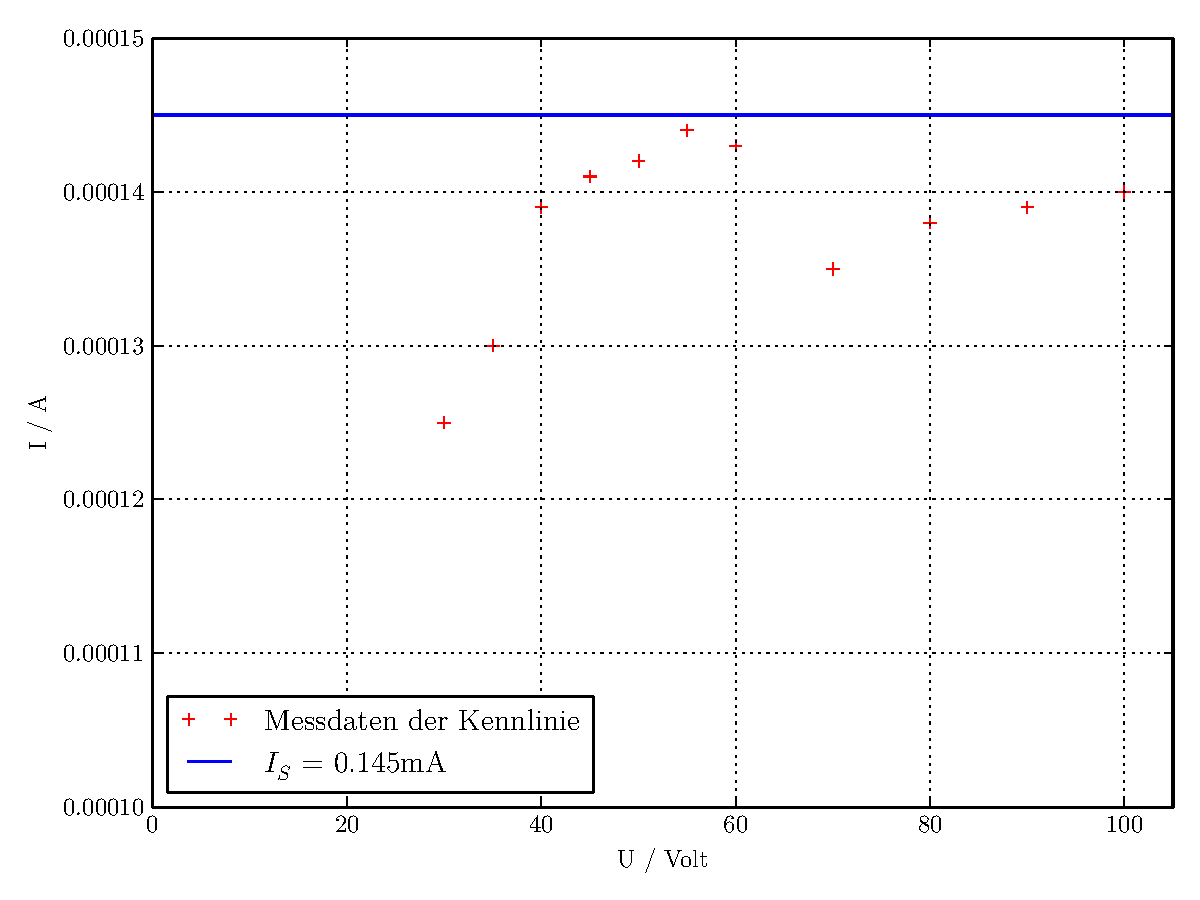
\includegraphics[width=0.9\textwidth]{build/Kennlinie1.pdf}
  \caption{Messdaten bei einer Heizspannung von 2V, und einem Heizstrom von 5A \cite{sample}}
  \label{fig:kenn1}
\end{figure}
Bei den beschriebenen Heizungseigenschaften (Abb. \ref{fig:kenn1}) liegt der Sättigungsstrom bei 
\begin{equation}
I_S = 0.145 \mathrm{mA}.
\label{eq:kenn1ergebnis}
\end{equation}


\begin{figure}[H]
  \centering
  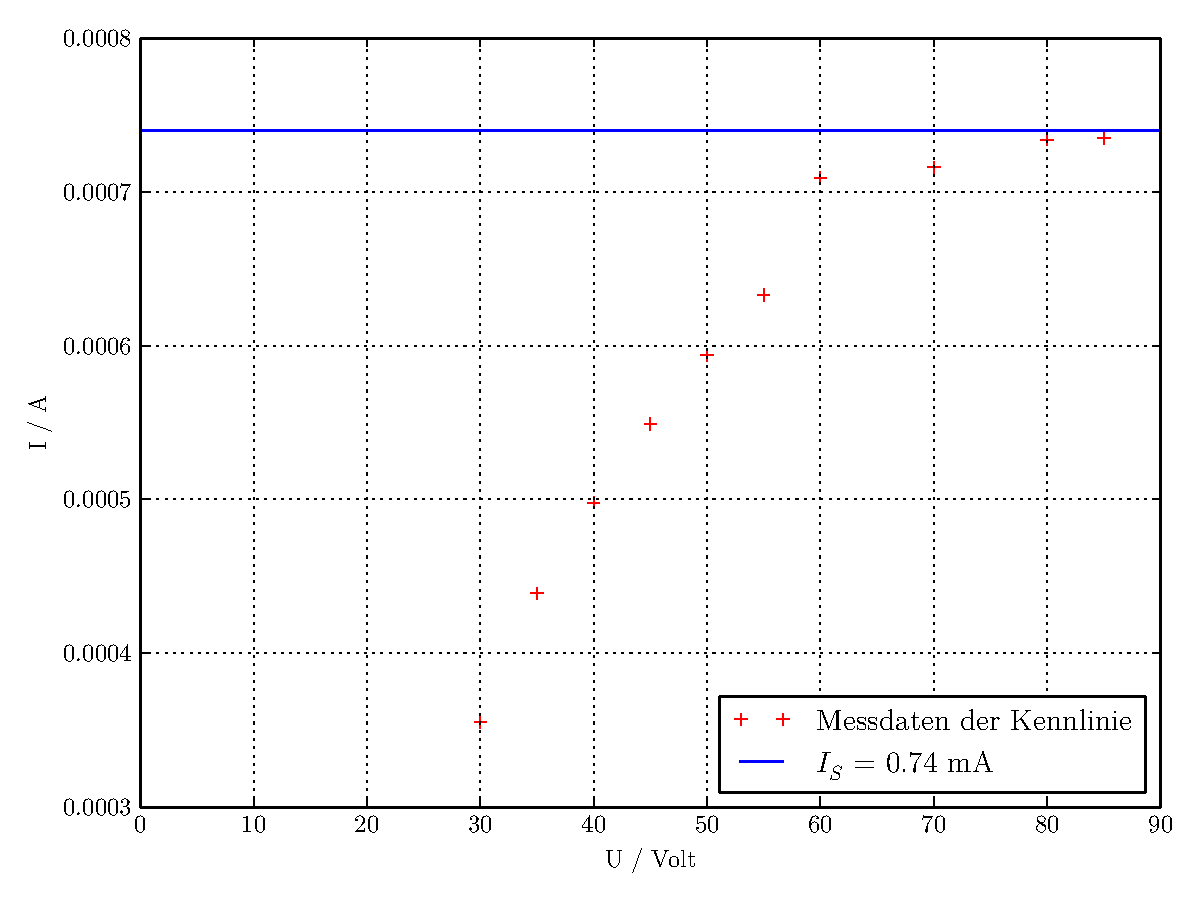
\includegraphics[width=0.8\textwidth]{build/Kennlinie2.pdf}
  \caption{Messdaten bei einer Heizspannung von 2.2V, und einem Heizstrom von 5.5A \cite{sample}}
  \label{fig:kenn2}
\end{figure}
Bei den beschriebenen Heizungseigenschaften (Abb. \ref{fig:kenn2}) liegt $I_S$ bei 
\begin{equation}
I_S = 0.74 \mathrm{mA}.
\label{eq:kenn2ergebnis}
\end{equation}


\begin{figure}[H]
  \centering
  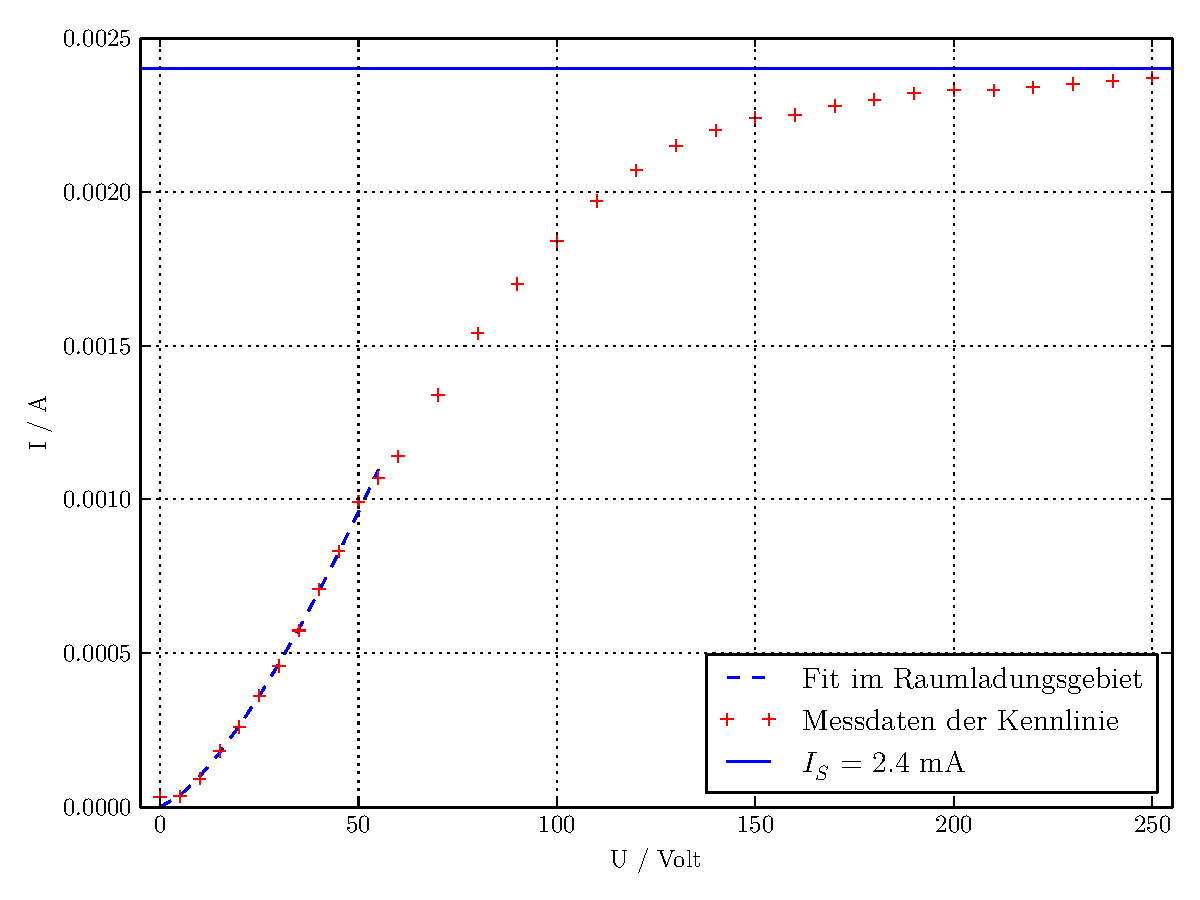
\includegraphics[width=0.8\textwidth]{build/Kennlinie4.pdf}
  \caption{Messdaten bei einer Heizspannung von 2.4V, und einem Heizstrom von 6A \cite{sample}}
  \label{fig:kenn4}
\end{figure}
Bei den beschriebenen Heizungseigenschaften (Abb. \ref{fig:kenn4}) liegt der Strom bei 
\begin{equation}
I_S = 2.4 \mathrm{mA}.
\label{eq:kenn4ergebnis}
\end{equation}
Der Raumladungsbereuch wurde nach Abbildung \ref{fig:6} abgeschätzt. In diesem Bereich wird
gegenüber den Daten ein Fit angelegt. Dies geschieht nach der Gleichung \eqref{eq:langmuir}. Der Exponent der Spannung U war dabei
der zu bestimmende Fitparameter der Fitfunktion $\mathrm{const} \cdot \frac{\mathrm{U}^b}{\mathrm{a}^2}$ . Er wurde mit NumPy \cite{numpy} als 1.407 bestimmt.



\subsection{Das Anlaufstromgebiet und die Temperatur}
\label{subsec:c}
Die Messdaten des Anlaufstromgebiets werden geplottet und es wird nach einer Spannungskorrektur eine Ausgleichskurve nach \eqref{eq:anlauf} angelegt.
\begin{figure}[H]
  \centering
  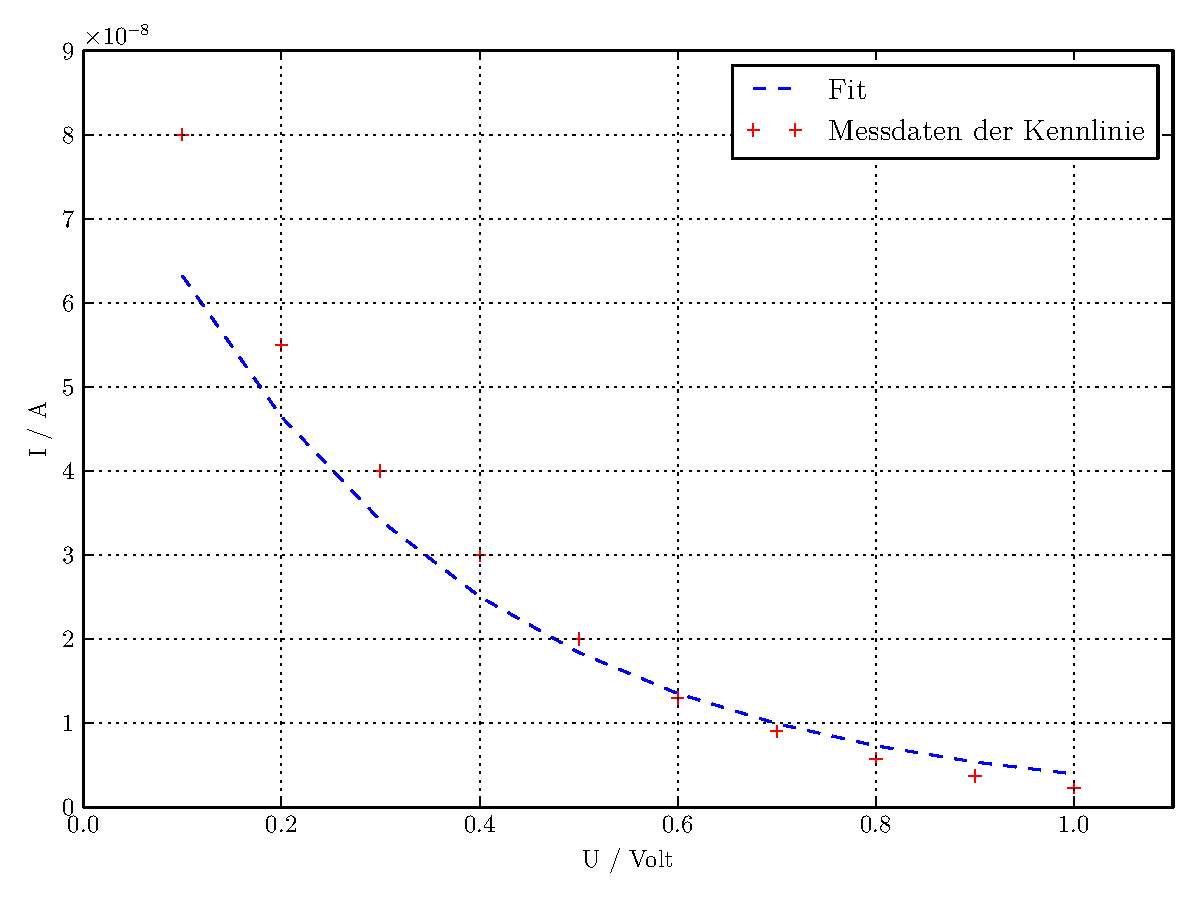
\includegraphics[width=0.9\textwidth]{build/Kennlinie3.pdf}
  \caption{Messdaten des Anlaufstromgebiets bei einer Heizspannung von 2.4V, und einem Heizstrom von 6A \cite{sample}}
  \label{fig:kenn3}
\end{figure}
Mit den herausgefundenen Parametern kommt man auf eine Temperatur von
$3761.16 \mathrm{K} \pm 2.897 \%$.


\subsection{Kathodentemperaturen}
\label{subsec:d}
Mit 
\begin{equation}
T = \sqrt[4]{\frac{I_H \cdot U_H - N_{WL}}{f \eta \sigma}}
\label{eq:kenn1ergebnis}
\end{equation}
\cite{sample} kann die Temperatur aus den gemessenen Wertepaaren in Unterkapitel \ref{subsec:kennlinien} errechnet werden.
Für die Heizung verwendet in Abbildung \ref{fig:kenn1} findet man so eine Temperatur von
$2048.87$ K. \\
Für die Daten in Abbildung \ref{fig:kenn2} findet man
$2159.16$ K. \\
Für die Daten in Abbildung \ref{fig:kenn4} findet man
$2263.24$ K. \\

\subsection{Austrittsarbeit}
\label{subsec:e}
Durch das Umstellen von Gl. \eqref{eq:richardson} ist es möglich, die Austrittsarbeit des verwendeten Materials 
(hier: Wolfram) auszurechnen. 
Die Austrittsarbeit beträgt demnach 3.82 eV für die Daten in \ref{fig:kenn1}. \\
Sie beträgt ca. 3.728 eV für die Kennlinie \ref{fig:kenn2}. \\
Die Austrittsarbeit der Kennlinie \ref{fig:kenn4} liegt bei 3.71 eV. \\
